\documentclass[letterpaper,10pt,addpoints]{exam}
\usepackage{graphicx}
\graphicspath{ {images/} }
\usepackage[utf8]{inputenc}
\usepackage{fontenc}
\usepackage{amsmath}
\usepackage{relsize}
\usepackage{xfrac}
\usepackage{amsfonts}
\usepackage{amssymb}
\usepackage{asymptote}

\begin{document}

\begin{Large}
\begin{center}
\fbox{\fbox{\parbox{5.5in}{\centering AIME Geometry Problems}}}
\end{center}
\end{Large}

 
\vspace{5mm}


\textbf{1. (AIME 1983 - P4) } A machine-shop cutting tool has the shape of a notched circle, as shown. The radius of the circle is $\sqrt{50}$ cm, the length of $AB$ is 6 cm, and that of $BC$ is 2 cm. The angle $ABC$ is a right angle. Find the square of the distance (in centimeters) from $B$ to the center of the circle.\quad  \textbf{Ans: 026}

\begin{center}
\begin{asy}
 size(100); defaultpen(linewidth(0.6)+fontsize(11)); real r=10; pair O=(0,0),A=r*dir(45),B=(A.x,A.y-r),C; path P=circle(O,r); C=intersectionpoint(B--(B.x+r,B.y),P); draw(P); draw(C--B--O--A--B); dot(O); dot(A); dot(B); dot(C); label("$O$",O,SW); label("$A$",A,NE); label("$B$",B,S); label("$C$",C,SE); 
\end{asy}
\end{center}

\textbf{2. (AIME 1983 - P11) } The solid shown has a square base of side length $s$. The upper edge is parallel to the base and has length $2s$. All other edges have length $s$. Given that  $s=6\sqrt{2}$, what is the volume of the solid?\quad  \textbf{Ans: 288}

\begin{center}
\begin{asy}
import cse5;
size(120); import three; pathpen = black+linewidth(0.65); pointpen = black; currentprojection = perspective(30,-20,10); real s = 6 * 2^.5; triple A=(0,0,0),B=(s,0,0),C=(s,s,0),D=(0,s,0),E=(-s/2,s/2,6),F=(3*s/2,s/2,6); draw(A--B--C--D--A--E--D); draw(B--F--C); draw(E--F); label("A",A,W); label("B",B,S); label("C",C,SE); label("D",D,NE); label("E",E,N); label("F",F,N);
\end{asy}
\end{center}

\textbf{3. (AIME 1983 - P12) } The length of diameter $AB$ is a two digit integer. Reversing the digits gives the length of a perpendicular chord $CD$. The distance from their intersection point $H$ to the center $O$ is a positive rational number. Determine the length of $AB$.\quad  \textbf{Ans: 065}

\begin{center}
\begin{asy}
import cse5;
size(120);
pointpen=black; pathpen=black+linewidth(0.65); pair O=(0,0),A=(-65/2,0),B=(65/2,0); pair H=(-((65/2)^2-28^2)^.5,0),C=(H.x,28),D=(H.x,-28); D(CP(O,A));D(MP("A",A,W)--MP("B",B,E));D(MP("C",C,N)--MP("D",D)); dot(MP("H",H,SE));dot(MP("O",O,SE)); 
\end{asy}
\end{center}

\textbf{4. (AIME 1983 - P14) } In the adjoining figure, two circles with radii $8$ and $6$ are drawn with their centers $12$ units apart. At $P$, one of the points of intersection, a line is drawn in such a way that the chords $QP$ and $PR$ have equal length. Find the square of the length of $QP$.\quad  \textbf{Ans: 130}

\begin{center}
\begin{asy}
import cse5;
import olympiad;
size(160); defaultpen(linewidth(.8pt)+fontsize(11pt)); dotfactor=3; pair O1=(0,0), O2=(12,0); path C1=Circle(O1,8), C2=Circle(O2,6); pair P=intersectionpoints(C1,C2)[0]; path C3=Circle(P,sqrt(130)); pair Q=intersectionpoints(C3,C1)[0]; pair R=intersectionpoints(C3,C2)[1]; draw(C1); draw(C2); draw(O2--O1); dot(O1); dot(O2); draw(Q--R); label("$Q$",Q,NW); label("$P$",P,1.5*dir(80)); label("$R$",R,NE); label("12",waypoint(O1--O2,0.4),S);
\end{asy}
\end{center}

\textbf{5. (AIME 1983 - P15) }The adjoining figure shows two intersecting chords in a circle, with $B$ on minor arc $AD$. Suppose that the radius of the circle is $5$, that $BC=6$, and that $AD$ is bisected by $BC$. Suppose further that $AD$ is the only chord starting at $A$ which is bisected by $BC$. It follows that the sine of the minor arc $AB$ is a rational number. If this fraction is expressed as a fraction $\frac{m}{n}$ in lowest terms, what is the product $mn$?\quad  \textbf{Ans: 175}

\begin{center}
\begin{asy}
import cse5;
import olympiad;
size(100); defaultpen(linewidth(.8pt)+fontsize(11pt)); dotfactor=1; pair O1=(0,0); pair A=(-0.91,-0.41); pair B=(-0.99,0.13); pair C=(0.688,0.728); pair D=(-0.25,0.97); path C1=Circle(O1,1); draw(C1); label("$A$",A,W); label("$B$",B,W); label("$C$",C,NE); label("$D$",D,N); draw(A--D); draw(B--C); pair F=intersectionpoint(A--D,B--C); add(pathticks(A--F,1,0.5,0,3.5)); add(pathticks(F--D,1,0.5,0,3.5)); 
\end{asy}
\end{center}

\textbf{6. (AIME 1984 - P3) }A point $P$ is chosen in the interior of $\triangle ABC$ such that when lines are drawn through $P$ parallel to the sides of $\triangle ABC$, the resulting smaller triangles $t_{1}$, $t_{2}$, and $t_{3}$ in the figure, have areas $4$, $9$, and $49$, respectively. Find the area of $\triangle ABC$.\quad  \textbf{Ans: 144}

\begin{center}
\begin{asy}
import cse5;
import olympiad;
size(200); pathpen=black;pointpen=black; pair A=(0,0),B=(12,0),C=(4,5); D(A--B--C--cycle); D(A+(B-A)*3/4--A+(C-A)*3/4); D(B+(C-B)*5/6--B+(A-B)*5/6);D(C+(B-C)*5/12--C+(A-C)*5/12); MP("A",C,N);MP("B",A,SW);MP("C",B,SE); /* sorry mixed up points according to resources diagram. */ MP("t_3",(A+B+(B-A)*3/4+(A-B)*5/6)/2+(-1,0.8),N); MP("t_2",(B+C+(B-C)*5/12+(C-B)*5/6)/2+(-0.3,0.1),WSW); MP("t_1",(A+C+(C-A)*3/4+(A-C)*5/12)/2+(0,0.15),ESE); 
\end{asy}
\end{center}

\textbf{7. (AIME 1984 - P9) }In tetrahedron $ABCD$, edge $AB$ has length 3 cm. The area of face $ABC$ is $15\mbox{cm}^2$ and the area of face $ABD$ is $12 \mbox { cm}^2$. These two faces meet each other at a $30^\circ$ angle. Find the volume of the tetrahedron in $\mbox{cm}^3$.\quad  \textbf{Ans: 020}

\begin{center}
\begin{asy}
import cse5;
import olympiad;
/* modified version of olympiad modules */
 import three; real markscalefactor = 0.03; path3 rightanglemark(triple A, triple B, triple C, real s=8) { 	triple P,Q,R; 	P=s*markscalefactor*unit(A-B)+B; 	R=s*markscalefactor*unit(C-B)+B; 	Q=P+R-B; 	return P--Q--R; } path3 anglemark(triple A, triple B, triple C, real t=8 ... real[] s) {  	triple M,N,P[],Q[];  	path3 mark;  	int n=s.length; 	M=t*markscalefactor*unit(A-B)+B;  	N=t*markscalefactor*unit(C-B)+B;  	for (int i=0; i<n; ++i)   	{   		P[i]=s[i]*markscalefactor*unit(A-B)+B;   		Q[i]=s[i]*markscalefactor*unit(C-B)+B;  	}  	mark=arc(B,M,N);  	for (int i=0; i<n; ++i)  	{   		if (i%2==0)   		{    			mark=mark--reverse(arc(B,P[i],Q[i]));   		}   		else   		{    			mark=mark--arc(B,P[i],Q[i]);    		}  	}  	if (n%2==0 && n!=0)  	mark=(mark--B--P[n-1]);  	else if (n!=0)  	mark=(mark--B--Q[n-1]);  	else mark=(mark--B--cycle);  	return mark; }  size(200); import three; defaultpen(black+linewidth(0.7)); pen small = fontsize(10); triple A=(0,0,0),B=(3,0,0),C=(1.8,10,0),D=(1.5,4,4),Da=(D.x,D.y,0),Db=(D.x,0,0);  currentprojection=perspective(16,-10,8);  draw(surface(A--B--C--cycle),rgb(0.6,0.7,0.6),nolight); draw(surface(A--B--D--cycle),rgb(0.7,0.6,0.6),nolight);  /* draw pyramid - other lines + angles */ draw(A--B--C--A--D--B--D--C);  draw(D--Da--Db--cycle); draw(rightanglemark(D,Da,Db));draw(rightanglemark(A,Db,D));draw(anglemark(Da,Db,D,15));  /* labeling points */ label("$A$",A,SW);label("$B$",B,S);label("$C$",C,S);label("$D$",D,N);label("$30^{\circ}$",Db+(0,.35,0.08),(1.5,1.2),small); label("$3$",(A+B)/2,S); label("$15\mathrm{cm}^2$",(Db+C)/2+(0,-0.5,-0.1),NE,small); label("$12\mathrm{cm}^2$",(A+D)/2,NW,small); 
\end{asy}
\end{center}

\textbf{8. (AIME 1985 - P2) }When a right triangle is rotated about one leg, the volume of the cone produced is $800\pi \;\textrm{ cm}^3$. When the triangle is rotated about the other leg, the volume of the cone produced is $1920\pi \;\textrm{ cm}^3$. What is the length (in cm) of the hypotenuse of the triangle?\quad  \textbf{Ans: 026}\\ 

\textbf{9. (AIME 1985 - P4) } A small square is constructed inside a square of area 1 by dividing each side of the unit square into $n$ equal parts, and then connecting the vertices to the division points closest to the opposite vertices. Find the value of $n$ if the the area of the small square is exactly $\mathlarger{\frac1{1985}}$.\quad  \textbf{Ans: 032}
\begin{center}
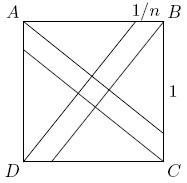
\includegraphics[scale=0.6]{AIME_1985_Problem_4.png}
\end{center}

\textbf{10. (AIME 1985 - P6) }As shown in the figure, triangle $ABC$ is divided into six smaller triangles by lines drawn from the vertices through a common interior point. The areas of four of these triangles are as indicated. Find the area of triangle $ABC$.\quad  \textbf{Ans: 315}
\begin{center}
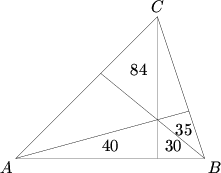
\includegraphics[scale=0.6]{AIME_1985_Problem_6.png}
\end{center}

\textbf{11. (AIME 1985 - P9) }In a circle, parallel chords of lengths 2, 3, and 4 determine central angles of $\alpha$, $\beta$, and $\alpha + \beta$ radians, respectively, where $\alpha + \beta < \pi$. If $\cos \alpha$, which is a positive rational number, is expressed as a fraction in lowest terms, what is the sum of its numerator and denominator?\quad  \textbf{Ans: 049}\\

\textbf{12. (AIME 1985 - P15) }Three 12 cm $\times$12 cm squares are each cut into two pieces $A$ and $B$, as shown in the first figure below, by joining the midpoints of two adjacent sides. These six pieces are then attached to a regular hexagon, as shown in the second figure, so as to fold into a polyhedron. What is the volume (in $\mathrm{cm}^3$) of this polyhedron?\quad  \textbf{Ans: 864}

\begin{center}
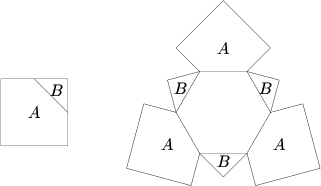
\includegraphics[scale=0.6]{AIME_1985_Problem_15.png}
\end{center}

\textbf{13. (AIME 1986 - P9) } In $\triangle ABC$, $AB= 425$, $BC=450$, and $AC=510$. An interior point $P$ is then drawn, and segments are drawn through $P$ parallel to the sides of the triangle. If these three segments are of an equal length $d$, find $d$.\quad  \textbf{Ans: 306}\\

\textbf{14. (AIME 1986 - P14) } The shortest distances between an interior diagonal of a rectangular parallelepiped, $P$, and the edges it does not meet are $\mathlarger{2\sqrt{5}}$, $\mathlarger{\frac{30}{\sqrt{13}}}$, and $\mathlarger{\frac{15}{\sqrt{10}}}$. Determine the volume of $P$.\textbf{Ans: 750}\\

\textbf{15. (AIME 1986 - P15) } Let triangle $ABC$ be a right triangle in the xy-plane with a right angle at $C_{}$. Given that the length of the hypotenuse $AB$ is $60$, and that the medians through $A$ and $B$ lie along the lines $y=x+3$ and $y=2x+4$ respectively, find the area of triangle $ABC$.\quad  \textbf{Ans: 400}\\

\textbf{16. (AIME 1987 - P6) } Rectangle $ABCD$ is divided into four parts of equal area by five segments as shown in the figure, where $XY = YB + BC + CZ = ZW = WD + DA + AX$, and $PQ$ is parallel to $AB$. Find the length of $AB$ (in cm) if $BC = 19$ cm and $PQ = 87$ cm.\quad  \textbf{Ans: 193}

\begin{center}
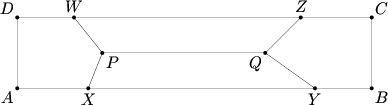
\includegraphics[scale=0.6]{AIME_1987_Problem_6.png}
\end{center}

\textbf{17. (AIME 1987 - P9) } Triangle $ABC$ has right angle at $B$, and contains a point $P$ for which $PA = 10$, $PB = 6$, and $\angle APB = \angle BPC = \angle CPA$. Find $PC$\quad  \textbf{Ans: 033}

\begin{center}
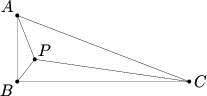
\includegraphics[scale=0.6]{AIME_1987_Problem_9.png}
\end{center}

\textbf{18. (AIME 1987 - P15) } Squares $S_1$ and $S_2$ are inscribed in right triangle $ABC$, as shown in the figures below. Find $AC + CB$ if area $(S_1) = 441$ and area $(S_2) = 440$.\quad  \textbf{Ans: 462}

\begin{center}
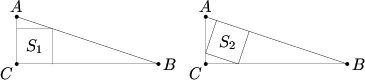
\includegraphics[scale=0.6]{AIME_1987_Problem_15.png}
\end{center}

\textbf{19. (AIME 1988 - P12) } Let $P$ be an interior point of triangle $ABC$ and extend lines from the vertices through $P$ to the opposite sides. Let $a$, $b$, $c$, and $d$ denote the lengths of the segments indicated in the figure. Find the product $abc$ if $a + b + c = 43$ and $d = 3$.\quad  \textbf{Ans: 441}

\begin{center}
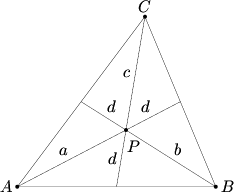
\includegraphics[scale=0.6]{1988_AIME-12.png}
\end{center}

\textbf{20. (AIME 1989 - P6) } Two skaters, Allie and Billie, are at points $A$ and $B$, respectively, on a flat, frozen lake. The distance between $A$ and $B$ is $100$ meters. Allie leaves $A$ and skates at a speed of $8$ meters per second on a straight line that makes a $60^\circ$ angle with $AB$. At the same time Allie leaves $A$, Billie leaves $B$ at a speed of $7$ meters per second and follows the straight path that produces the earliest possible meeting of the two skaters, given their speeds. How many meters does Allie skate before meeting Billie? \textbf{Ans: 160}

\begin{center}
\begin{asy}
import cse5;
import olympiad;
size(200);
pointpen=black; pathpen=black+linewidth(0.7);  pair A=(0,0),B=(10,0),C=6*expi(pi/3); D(B--A); D(A--C,EndArrow); MP("A",A,SW);MP("B",B,SE);MP("60^{\circ}",A+(0.3,0),NE);MP("100",(A+B)/2); 
\end{asy}
\end{center}

\textbf{21. (AIME 1989 - P10) } Let $a$, $b$, $c$ be the three sides of a triangle, and let $\alpha$, $\beta$, $\gamma$, be the angles opposite them. If $a^2+b^2=1989c^2$, find $\mathlarger{\frac{\cot \gamma}{\cot \alpha+\cot \beta}}$ \quad  \textbf{Ans: 994}\\

\textbf{22. (AIME 1989 - P12) }Let $ABCD$ be a tetrahedron with $AB=41$, $AC=7$, $AD=18$, $BC=36$, $BD=27$, and $CD=13$, as shown in the figure. Let $d$ be the distance between the midpoints of edges $AB$ and $CD$. Find $d^{2}$.\quad  \textbf{Ans: 137}

\begin{center}
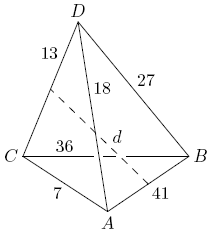
\includegraphics[scale=0.6]{AIME_1989_Problem_12.png}
\end{center}

\textbf{23. (AIME 1989 - P15) }Point $P$ is inside $\triangle ABC$. Line segments $APD$, $BPE$, and $CPF$ are drawn with $D$ on $BC$, $E$ on $AC$, and $F$ on $AB$ (see the figure below). Given that $AP=6$, $BP=9$, $PD=6$, $PE=3$, and $CF=20$, find the area of $\triangle ABC$.\quad  \textbf{Ans: 108}

\begin{center}
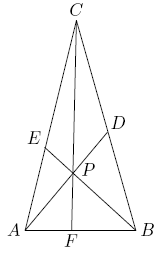
\includegraphics[scale=0.6]{AIME_1989_Problem_15.png}
\end{center}

\textbf{24. (AIME 1990 - P3) }Let $P_1^{}$ be a regular $r~\mbox{gon}$ and $P_2^{}$ be a regular $s~\mbox{gon}$ $(r\geq s\geq 3)$ such that each interior angle of $P_1^{}$ is $\frac{59}{58}$ as large as each interior angle of $P_2^{}$. What's the largest possible value of $s_{}^{}$?\quad  \textbf{Ans: 117}\\

\textbf{25. (AIME 1990 - P7) }A triangle has vertices $P_{}^{}=(-8,5)$, $Q_{}^{}=(-15,-19)$, and $R_{}^{}=(1,-7)$. The equation of the bisector of $\angle P$ can be written in the form $ax+2y+c=0_{}^{}$. Find $a+c_{}^{}$.\quad  \textbf{Ans: 89}

\begin{center}
\begin{asy}
import cse5;
import olympiad;
import graph;
size(100);
pointpen=black;pathpen=black+linewidth(0.7);pen f = fontsize(10); pair P=(-8,5),Q=(-15,-19),R=(1,-7),S=(7,-15),T=(-4,-17); MP("P",P,N,f);MP("Q",Q,W,f);MP("R",R,E,f); D(P--Q--R--cycle);D(P--T,EndArrow(2mm)); D((-17,0)--(4,0),Arrows(2mm));D((0,-21)--(0,7),Arrows(2mm)); 
\end{asy}
\end{center}

\textbf{26. (AIME 1990 - P12) }A regular 12-gon is inscribed in a circle of radius 12. The sum of the lengths of all sides and diagonals of the 12-gon can be written in the form $a + b \sqrt{2} + c \sqrt{3} + d \sqrt{6},$ where $a^{}_{}$, $b^{}_{}$, $c^{}_{}$, and $d^{}_{}$ are positive integers. Find $a + b + c + d^{}_{}$.\quad  \textbf{Ans: 720}\\

\textbf{27. (AIME 1990 - P14) }The rectangle $ABCD^{}_{}$ below has dimensions $AB^{}_{} = 12 \sqrt{3}$ and $BC^{}_{} = 13 \sqrt{3}$. Diagonals $\overline{AC}$ and $\overline{BD}$ intersect at $P^{}_{}$. If triangle $ABP^{}_{}$ is cut out and removed, edges $\overline{AP}$ and $\overline{BP}$ are joined, and the figure is then creased along segments $\overline{CP}$ and $\overline{DP}$, we obtain a triangular pyramid, all four of whose faces are isosceles triangles. Find the volume of this pyramid.\quad  \textbf{Ans: 594}

\begin{center}
\begin{asy}
import cse5;
import olympiad;
import graph;
size(150);
 pair D=origin, A=(13,0), B=(13,12), C=(0,12), P=(6.5, 6); draw(B--C--P--D--C^^D--A); filldraw(A--P--B--cycle, gray, black); label("$A$", A, SE); label("$B$", B, NE); label("$C$", C, NW); label("$D$", D, SW); label("$P$", P, N); label("$13\sqrt{3}$", A--D, S); label("$12\sqrt{3}$", A--B, E);
\end{asy}
\end{center}

\textbf{28. (AIME 1991 - P2) }Rectangle $ABCD_{}^{}$ has sides $\overline {AB}$ of length 4 and $\overline {CB}$ of length 3. Divide $\overline {AB}$ into 168 congruent segments with points $A_{}^{}=P_0, P_1, \ldots, P_{168}=B$, and divide $\overline {CB}$ into 168 congruent segments with points $C_{}^{}=Q_0, Q_1, \ldots, Q_{168}=B$. For $1_{}^{} \le k \le 167$, draw the segments $\overline {P_kQ_k}$. Repeat this construction on the sides $\overline {AD}$ and $\overline {CD}$, and then draw the diagonal $\overline {AC}$. Find the sum of the lengths of the 335 parallel segments drawn.\quad  \textbf{Ans: 840}\\

\textbf{29. (AIME 1991 - P11) }Twelve congruent disks are placed on a circle $C^{}_{}$ of radius 1 in such a way that the twelve disks cover $C^{}_{}$, no two of the disks overlap, and so that each of the twelve disks is tangent to its two neighbors. The resulting arrangement of disks is shown in the figure below. The sum of the areas of the twelve disks can be written in the from $\pi(a-b\sqrt{c})$, where $a,b,c^{}_{}$ are positive integers and $c^{}_{}$ is not divisible by the square of any prime. Find $a+b+c^{}_{}$.\quad  \textbf{Ans: 135}

\begin{center}
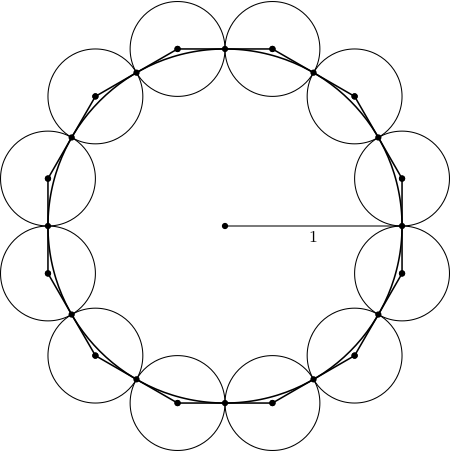
\includegraphics[scale=0.6]{AIME_1991_Problem_11.png}
\end{center}

\textbf{30. (AIME 1991 - P12) }Rhombus $PQRS^{}_{}$ is inscribed in rectangle $ABCD^{}_{}$ so that vertices $P^{}_{}$, $Q^{}_{}$, $R^{}_{}$, and $S^{}_{}$ are interior points on sides $\overline{AB}$, $\overline{BC}$, $\overline{CD}$, and $\overline{DA}$, respectively. It is given that $PB^{}_{}=15$, $BQ^{}_{}=20$, $PR^{}_{}=30$, and $QS^{}_{}=40$. Let $m/n^{}_{}$, in lowest terms, denote the perimeter of $ABCD^{}_{}$. Find $m+n^{}_{}$.\textbf{Ans: 677}\\

\textbf{31. (AIME 1991 - P14) }A hexagon is inscribed in a circle. Five of the sides have length $81$ and the sixth, denoted by $\overline{AB}$, has length $31$. Find the sum of the lengths of the three diagonals that can be drawn from $A_{}^{}$.\quad\textbf{Ans: 384}\\

\textbf{32. (AIME 1992 - P9) }Trapezoid $ABCD^{}_{}$ has sides $AB=92^{}_{}$, $BC=50^{}_{}$, $CD=19^{}_{}$, and $AD=70^{}_{}$, with $AB^{}_{}$ parallel to $CD^{}_{}$. A circle with center $P^{}_{}$ on $AB^{}_{}$ is drawn tangent to $BC^{}_{}$ and $AD^{}_{}$. Given that $AP=\dfrac{m}{n}$, where $m^{}_{}$ and $n^{}_{}$ are relatively prime positive integers, find $m+n^{}_{}$.\quad\textbf{Ans:}$ \dfrac{161}{3}$\\

\textbf{33. (AIME 1992 - P11) }Lines $l_1^{}$ and $l_2^{}$ both pass through the origin and make first-quadrant angles of $\dfrac{\pi}{70}$ and $\dfrac{\pi}{54}$ radians, respectively, with the positive x-axis. For any line $l^{}_{}$, the transformation $R(l)^{}_{}$ produces another line as follows: $l^{}_{}$ is reflected in $l_1^{}$, and the resulting line is reflected in $l_2^{}$. Let $R^{(1)}(l)=R(l)^{}_{}$ and $R^{(n)}(l)^{}_{}=R\left(R^{(n-1)}(l)\right)$. Given that $l^{}_{}$ is the line $y=\dfrac{19}{92}x^{}_{}$, find the smallest positive integer $m^{}_{}$ for which $R^{(m)}(l)=l^{}_{}$.\quad\textbf{Ans: 945}\\

\textbf{34. (AIME 1992 - P13) }Triangle $ABC$ has $AB=9$ and $BC: AC=40: 41$. What's the largest area that this triangle can have?\quad\textbf{Ans: 820}\\

\textbf{35. (AIME 1992 - P14) }In triangle $ABC^{}_{}$, $A'$, $B'$, and $C'$ are on the sides $BC$, $AC^{}_{}$, and $AB^{}_{}$, respectively. Given that $AA'$, $BB'$, and $CC'$ are concurrent at the point $O^{}_{}$, and that $\mathlarger{\frac{AO^{}_{}}{OA'}+\frac{BO}{OB'}+\frac{CO}{OC'}=92}$, find $\mathlarger{\frac{AO}{OA'}\cdot \frac{BO}{OB'}\cdot \frac{CO}{OC'}}$.\quad\textbf{Ans: 94}\\

\textbf{36. (AIME 1993 - P13) }Jenny and Kenny are walking in the same direction, Kenny at 3 feet per second and Jenny at 1 foot per second, on parallel paths that are 200 feet apart. A tall circular building 100 feet in diameter is centered midway between the paths. At the instant when the building first blocks the line of sight between Jenny and Kenny, they are 200 feet apart. Let $t\,$ be the amount of time, in seconds, before Jenny and Kenny can see each other again. If $t\,$ is written as a fraction in lowest terms, what is the sum of the numerator and denominator?\quad\textbf{Ans: 163}\\

\textbf{37. (AIME 1993 - P15) }Let $\overline{CH}$ be an altitude of $\triangle ABC$. Let $R\,$ and $S\,$ be the points where the circles inscribed in the triangles $ACH\,$ and $BCH^{}_{}$ are tangent to $\overline{CH}$. If $AB = 1995\,$, $AC = 1994\,$, and $BC = 1993\,$, then $RS\,$ can be expressed as $m/n\,$, where $m\,$ and $n\,$ are relatively prime integers. Find $m + n\,$.\quad\textbf{Ans: 997}\\

\textbf{38. (AIME 1994 - P2) }A circle with diameter $\overline{PQ}$ of length 10 is internally tangent at $P$ to a circle of radius 20. Square $ABCD$ is constructed with $A$ and $B$ on the larger circle, $\overline{CD}$ tangent at $Q$ to the smaller circle, and the smaller circle outside $ABCD$. The length of $\overline{AB}$ can be written in the form $m + \sqrt{n}$, where $m$ and $n$ are integers. Find $m + n$.\quad\textbf{Ans: 312}

\begin{center}
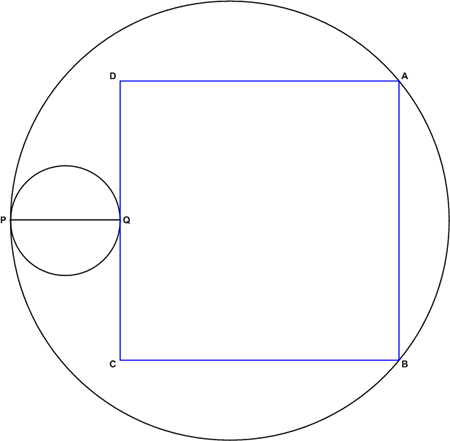
\includegraphics[scale=0.4]{AIME_1994_Problem_2.png}
\end{center}

\textbf{39. (AIME 1994 - P6) }The graphs of the equations $y=k, \quad y=\sqrt{3}x+2k, \quad y=-\sqrt{3}x+2k,$ are drawn in the coordinate plane for $k=-10,-9,-8,\ldots,9,10.\,$ These 63 lines cut part of the plane into equilateral triangles of side $2/\sqrt{3}.\,$ How many such triangles are formed?\quad\textbf{Ans: 660}\\

\textbf{40. (AIME 1994 - P8) }The points $(0,0)\,$, $(a,11)\,$, and $(b,37)\,$ are the vertices of an equilateral triangle. Find the value of $ab\,$.\quad\textbf{Ans: 315}\\

\textbf{41. (AIME 1994 - P10) }In triangle $ABC,\,$ angle $C$ is a right angle and the altitude from $C\,$ meets $\overline{AB}\,$ at $D.\,$ The lengths of the sides of $\triangle ABC\,$ are integers, $BD=29^3,\,$ and $\cos B=m/n\,$, where $m\,$ and $n\,$ are relatively prime positive integers. Find $m+n.\,$\quad\textbf{Ans: 450}\\

\textbf{42. (AIME 1994 - P12) }A fenced, rectangular field measures $24$ meters by $52$ meters. An agricultural researcher has 1994 meters of fence that can be used for internal fencing to partition the field into congruent, square test plots. The entire field must be partitioned, and the sides of the squares must be parallel to the edges of the field. What is the largest number of square test plots into which the field can be partitioned using all or some of the 1994 meters of fence?\quad\textbf{Ans: 702}\\

\textbf{43. (AIME 1994 - P14) }A beam of light strikes $\overline{BC}\,$ at point $C\,$ with angle of incidence $\alpha=19.94^\circ\,$ and reflects with an equal angle of reflection as shown. The light beam continues its path, reflecting off line segments $\overline{AB}\,$ and $\overline{BC}\,$ according to the rule: angle of incidence equals angle of reflection. Given that $\beta=\alpha/10=1.994^\circ\,$ and $AB=BC,\,$ determine the number of times the light beam will bounce off the two line segments. Include the first reflection at $C\,$ in your count.\quad\textbf{Ans: 071}

\begin{center}
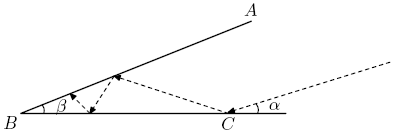
\includegraphics[scale=0.6]{AIME_1994_Problem_14.png}
\end{center}

\textbf{44. (AIME 1994 - P15) }Given a point $P^{}_{}$ on a triangular piece of paper $ABC,\,$ consider the creases that are formed in the paper when $A, B,\,$ and $C\,$ are folded onto $P.\,$ Let us call $P_{}^{}$ a fold point of $\triangle ABC\,$ if these creases, which number three unless $P^{}_{}$ is one of the vertices, do not intersect. Suppose that $AB=36, AC=72,\,$ and $\angle B=90^\circ.\,$ Then the area of the set of all fold points of $\triangle ABC\,$ can be written in the form $q\pi-r\sqrt{s},\,$ where $q, r,\,$ and $s\,$ are positive integers and $s\,$ is not divisible by the square of any prime. What is $q+r+s\,$?\quad\textbf{Ans: 597}\\

\textbf{45. (AIME 1995 - P4) }Circles of radius $3$ and $6$ are externally tangent to each other and are internally tangent to a circle of radius $9$. The circle of radius $9$ has a chord that is a common external tangent of the other two circles. Find the square of the length of this chord.\quad\textbf{Ans: 224}

\begin{center}
\begin{asy}
import cse5;
import olympiad;
import graph;
size(150);
pointpen = black; pathpen = black + linewidth(0.7); size(150); pair A=(0,0), B=(6,0), C=(-3,0), D=C+6*expi(acos(1/3)), F=B+3*expi(acos(1/3)), P=IP(F--F+3*(D-F),CR(A,9)), Q=IP(F--F+3*(F-D),CR(A,9)); D(CR(A,9)); D(CR(B,3)); D(CR(C,6)); D(P--Q); 
\end{asy}
\end{center}

\textbf{46. (AIME 1995 - P9) }Triangle $ABC$ is isosceles, with $AB=AC$ and altitude $AM=11.$ Suppose that there is a point $D$ on $\overline{AM}$ with $AD=10$ and $\angle BDC=3\angle BAC.$ Then the perimeter of $\triangle ABC$ may be written in the form $a+\sqrt{b},$ where $a$ and $b$ are integers. Find $a+b.$\quad\textbf{Ans: 616}

\begin{center}
\begin{asy}
import cse5;
import olympiad;
import graph;
size(3.5cm); real lsf=0.5; pen dps=linewidth(0.7)+fontsize(10); defaultpen(dps); pen ds=black; real xmin=-1.55,xmax=7.95,ymin=-4.41,ymax=5.3;  draw((1,3)--(0,0)); draw((0,0)--(2,0)); draw((2,0)--(1,3)); draw((1,3)--(1,0)); draw((1,0.7)--(0,0)); draw((1,0.7)--(2,0)); label("$11$",(1,1.63),W);  dot((1,3),ds); label("$A$",(1,3),N); dot((0,0),ds); label("$B$",(0,0),SW); dot((2,0),ds); label("$C$",(2,0),SE); dot((1,0),ds); label("$M$",(1,0),S); dot((1,0.7),ds); label("$D$",(1,0.7),NE);  clip((xmin,ymin)--(xmin,ymax)--(xmax,ymax)--(xmax,ymin)--cycle);
\end{asy}
\end{center}

\textbf{47. (AIME 1995 - P12)} Pyramid $OABCD$ has square base $ABCD,$ congruent edges $\overline{OA}, \overline{OB}, \overline{OC},$ and $\overline{OD},$ and $\angle AOB=45^\circ.$ Let $\theta$ be the measure of the dihedral angle formed by faces $OAB$ and $OBC.$ Given that $\cos \theta=m+\sqrt{n},$ where $m_{}$ and $n_{}$ are integers, find $m+n.$\quad\textbf{Ans: 005}\\

\textbf{48. (AIME 1995 - P14)} In a circle of radius $42$, two chords of length $78$ intersect at a point whose distance from the center is $18$. The two chords divide the interior of the circle into four regions. Two of these regions are bordered by segments of unequal lengths, and the area of either of them can be expressed uniquely in the form $m\pi-n\sqrt{d},$ where $m, n,$ and $d_{}$ are positive integers and $d_{}$ is not divisible by the square of any prime number. Find $m+n+d.$\quad\textbf{Ans: 378}\\

\textbf{49. (AIME 1996 - P4) }A wooden cube, whose edges are one centimeter long, rests on a horizontal surface. Illuminated by a point source of light that is $x$ centimeters directly above an upper vertex, the cube casts a shadow on the horizontal surface. The area of the shadow, which does not include the area beneath the cube is 48 square centimeters. Find the greatest integer that does not exceed $1000x$.\quad\textbf{Ans: 146}\\

\textbf{50. (AIME 1996 - P13) }In triangle $ABC$, $AB=\sqrt{30}$, $AC=\sqrt{6}$, and $BC=\sqrt{15}$. There is a point $D$ for which $\overline{AD}$ bisects $\overline{BC}$, and $\angle ADB$ is a right angle. The ratio $\dfrac{[ADB]}{[ABC]}$ can be written in the form $\dfrac{m}{n}$, where $m$ and $n$ are relatively prime positive integers. Find $m+n$.\quad\textbf{Ans: 065}\\

\textbf{51. (AIME 1996 - P14) }A $150\times 324\times 375$ rectangular solid is made by gluing together $1\times 1\times 1$ cubes. An internal diagonal of this solid passes through the interiors of how many of the $1\times 1\times 1$ cubes?\quad\textbf{Ans: 768}\\

\textbf{52. (AIME 1996 - P15) }In parallelogram $ABCD$, let $O$ be the intersection of diagonals $\overline{AC}$ and $\overline{BD}$. Angles $CAB$ and $DBC$ are each twice as large as angle $DBA$, and angle $ACB$ is $r$ times as large as angle $AOB$. Find the greatest integer that does not exceed $1000r$.\quad\textbf{Ans: 777}\\

\textbf{53. (AIME 1997 - P4) }Circles of radii $5, 5, 8,$ and $\dfrac mn$ are mutually externally tangent, where $m$ and $n$ are relatively prime positive integers. Find $m + n.$\quad\textbf{Ans: 017}\\

\textbf{54. (AIME 1997 - P6) }Point $B$ is in the exterior of the regular $n$-sided polygon $A_1A_2\cdots A_n$, and $A_1A_2B$ is an equilateral triangle. What is the largest value of $n$ for which $A_1$, $A_n$, and $B$ are consecutive vertices of a regular polygon?\quad\textbf{Ans: 042}\\

\textbf{55. (AIME 1997 - P7) }A car travels due east at $\frac 23$ mile per minute on a long, straight road. At the same time, a circular storm, whose radius is $51$ miles, moves southeast at $\frac 12\sqrt{2}$ mile per minute. At time $t=0$, the center of the storm is $110$ miles due north of the car. At time $t=t_1$ minutes, the car enters the storm circle, and at time $t=t_2$ minutes, the car leaves the storm circle. Find $\frac 12(t_1+t_2)$.\quad\textbf{Ans: 198}\\

\textbf{56. (AIME 1997 - P15) }The sides of rectangle $ABCD$ have lengths $10$ and $11$. An equilateral triangle is drawn so that no point of the triangle lies outside $ABCD$. The maximum possible area of such a triangle can be written in the form $p\sqrt{q}-r$, where $p$, $q$, and $r$ are positive integers, and $q$ is not divisible by the square of any prime number. Find $p+q+r$.\quad\textbf{Ans: 554}\\

\textbf{57. (AIME 1998 - P6) }Let $ABCD$ be a parallelogram. Extend $\overline{DA}$ through $A$ to a point $P,$ and let $\overline{PC}$ meet $\overline{AB}$ at $Q$ and $\overline{DB}$ at $R.$ Given that $PQ = 735$ and $QR = 112,$ find $RC.$\quad\textbf{Ans: 308}\\

\textbf{58. (AIME 1998 - P10) }Eight spheres of radius 100 are placed on a flat surface so that each sphere is tangent to two others and their centers are the vertices of a regular octagon. A ninth sphere is placed on the flat surface so that it is tangent to each of the other eight spheres. The radius of this last sphere is $a +b\sqrt {c},$ where $a, b,$ and $c$ are positive integers, and $c$ is not divisible by the square of any prime. Find $a + b + c$.\quad\textbf{Ans: 152}\\

\textbf{59. (AIME 1998 - P11) }Three of the edges of a cube are $\overline{AB}, \overline{BC},$ and $\overline{CD},$ and $\overline{AD}$ is an interior diagonal. Points $P, Q,$ and $R$ are on $\overline{AB}, \overline{BC},$ and $\overline{CD},$ respectively, so that $AP = 5, PB = 15, BQ = 15,$ and $CR = 10.$ What is the area of the polygon that is the intersection of plane $PQR$ and the cube?\textbf{Ans: 525}\\

\textbf{60. (AIME 1998 - P12) }Let $ABC$ be equilateral, and $D, E,$ and $F$ be the midpoints of $\overline{BC}, \overline{CA},$ and $\overline{AB},$ respectively. There exist points $P, Q,$ and $R$ on $\overline{DE}, \overline{EF},$ and $\overline{FD},$ respectively, with the property that $P$ is on $\overline{CQ}, Q$ is on $\overline{AR},$ and $R$ is on $\overline{BP}.$ The ratio of the area of triangle $ABC$ to the area of triangle $PQR$ is $a + b\sqrt {c},$ where $a, b$ and $c$ are integers, and $c$ is not divisible by the square of any prime. What is $a^{2} + b^{2} + c^{2}$?\quad\textbf{Ans: 083}\\

\textbf{61. (AIME 1999 - P2) }Consider the parallelogram with vertices $(10,45)$, $(10,114)$, $(28,153)$, and $(28,84)$. A line through the origin cuts this figure into two congruent polygons. The slope of the line is $m/n,$ where $m_{}$ and $n_{}$ are relatively prime positive integers. Find $m+n$.\quad\textbf{Ans: 118}\\

\textbf{62. (AIME 1999 - P4) }The two squares shown share the same center $O_{}$ and have sides of length 1. The length of $\overline{AB}$ is $43/99$ and the area of octagon $ABCDEFGH$ is  $m/n,$ where $m_{}$ and $n_{}$ are relatively prime positive integers. Find $m+n.$\quad\textbf{Ans: 185}

\begin{center}
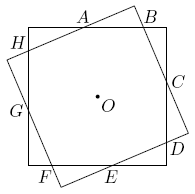
\includegraphics[scale=0.6]{AIME_1999_Problem_4.png}
\end{center}

\textbf{63. (AIME 1999 - P6) }A transformation of the first quadrant of the coordinate plane maps each point $(x,y)$ to the point $(\sqrt{x},\sqrt{y}).$ The vertices of quadrilateral $ABCD$ are $A=(900,300), B=(1800,600), C=(600,1800),$ and $D=(300,900).$ Let $k_{}$ be the area of the region enclosed by the image of quadrilateral $ABCD.$ Find the greatest integer that does not exceed $k_{}.$\quad\textbf{Ans: 314}\\

\textbf{64. (AIME 1999 - P12) }The inscribed circle of triangle $ABC$ is tangent to $\overline{AB}$ at $P_{},$ and its radius is $21$. Given that $AP=23$ and $PB=27,$ find the perimeter of the triangle.\quad\textbf{Ans: 345}\\

\textbf{65. (AIME 1999 - P14) }Point $P_{}$ is located inside triangle $ABC$ so that angles $PAB, PBC,$ and $PCA$ are all congruent. The sides of the triangle have lengths $AB=13, BC=14,$ and $CA=15,$ and the tangent of angle $PAB$ is $m/n,$ where $m_{}$ and $n_{}$ are relatively prime positive integers. Find $m+n.$\quad\textbf{Ans: 463}\\

\textbf{66. (AIME 1999 - P15) }Consider the paper triangle whose vertices are $(0,0), (34,0),$ and $(16,24).$ The vertices of its midpoint triangle are the midpoints of its sides. A triangular pyramid is formed by folding the triangle along the sides of its midpoint triangle. What is the volume of this pyramid?\quad\textbf{Ans: 408}\\

\textbf{67. (AIME I 2000 - P4) }The diagram shows a rectangle that has been dissected into nine non-overlapping squares. Given that the width and the height of the rectangle are relatively prime positive integers, find the perimeter of the rectangle.\quad\textbf{Ans: 260}

\begin{center}
\begin{asy}
import cse5;
import olympiad;
import graph;
size(100);
draw((0,0)--(69,0)--(69,61)--(0,61)--(0,0));draw((36,0)--(36,36)--(0,36)); draw((36,33)--(69,33));draw((41,33)--(41,61));draw((25,36)--(25,61)); draw((34,36)--(34,45)--(25,45)); draw((36,36)--(36,38)--(34,38)); draw((36,38)--(41,38)); draw((34,45)--(41,45));
\end{asy}
\end{center}

\textbf{68. (AIME I 2000  - P8) }A container in the shape of a right circular cone is $12$ inches tall and its base has a $5$-inch radius. The liquid that is sealed inside is $9$ inches deep when the cone is held with its point down and its base horizontal. When the liquid is held with its point up and its base horizontal, the height of the liquid is $m - n\sqrt [3]{p},$ from the base where $m,$ $n,$ and $p$ are positive integers and $p$ is not divisible by the cube of any prime number. Find $m + n + p$.\quad\textbf{Ans: 052}\\

\textbf{69. (AIME I 2000 - P13)} In the middle of a vast prairie, a firetruck is stationed at the intersection of two perpendicular straight highways. The truck travels at $50$ miles per hour along the highways and at $14$ miles per hour across the prairie. Consider the set of points that can be reached by the firetruck within six minutes. The area of this region is $m/n$ square miles, where $m$ and $n$ are relatively prime positive integers. Find $m + n$.\quad\textbf{Ans: 731}\\

\textbf{70. (AIME I 2000 - P14) }In triangle $ABC,$ it is given that angles $B$ and $C$ are congruent. Points $P$ and $Q$ lie on $\overline{AC}$ and $\overline{AB},$ respectively, so that $AP = PQ = QB = BC.$ Angle $ACB$ is $r$ times as large as angle $APQ,$ where $r$ is a positive real number. Find the greatest integer that does not exceed $1000r$.\quad\textbf{Ans: 571}\\

\textbf{71. (AIME 2000 II - P6) }One base of a trapezoid is $100$ units longer than the other base. The segment that joins the midpoints of the legs divides the trapezoid into two regions whose areas are in the ratio $2: 3$. Let $x$ be the length of the segment joining the legs of the trapezoid that is parallel to the bases and that divides the trapezoid into two regions of equal area. Find the greatest integer that does not exceed $x^2/100$.\quad\textbf{Ans: 181}\\

\textbf{72. (AIME 2000 II - P8) }In trapezoid $ABCD$, leg $\overline{BC}$ is perpendicular to bases $\overline{AB}$ and $\overline{CD}$, and diagonals $\overline{AC}$ and $\overline{BD}$ are perpendicular. Given that $AB=\sqrt{11}$ and $AD=\sqrt{1001}$, find $BC^2$.\quad\textbf{Ans: 017}\\

\textbf{73. (AIME 2000 II - P10) }A circle is inscribed in quadrilateral $ABCD$, tangent to $\overline{AB}$ at $P$ and to $\overline{CD}$ at $Q$. Given that $AP=19$, $PB=26$, $CQ=37$, and $QD=23$, find the square of the radius of the circle.\quad\textbf{Ans: 647}\\

\textbf{74. (AIME 2000 II - P11) }The coordinates of the vertices of isosceles trapezoid $ABCD$ are all integers, with $A=(20,100)$ and $D=(21,107)$. The trapezoid has no horizontal or vertical sides, and $\overline{AB}$ and $\overline{CD}$ are the only parallel sides. The sum of the absolute values of all possible slopes for $\overline{AB}$ is $m/n$, where $m$ and $n$ are relatively prime positive integers. Find $m+n$.\quad\textbf{Ans: 131}\\

\textbf{75. (AIME 2000 II - P12) }The points $A$, $B$ and $C$ lie on the surface of a sphere with center $O$ and radius $20$. It is given that $AB=13$, $BC=14$, $CA=15$, and that the distance from $O$ to $\triangle ABC$ is $\dfrac{m\sqrt{n}}k$, where $m$, $n$, and $k$ are positive integers, $m$ and $k$ are relatively prime, and $n$ is not divisible by the square of any prime. Find $m+n+k$\quad\textbf{Ans: 118}\\

\textbf{76. (AIME 2001 I - P4) }In triangle $ABC$, angles $A$ and $B$ measure $60$ degrees and $45$ degrees, respectively. The bisector of angle $A$ intersects $\overline{BC}$ at $T$, and $AT=24$. The area of triangle $ABC$ can be written in the form $a+b\sqrt{c}$, where $a$, $b$, and $c$ are positive integers, and $c$ is not divisible by the square of any prime. Find $a+b+c$.\quad\textbf{Ans: 291}\\

\textbf{77. (AIME 2001 I - P5) }An equilateral triangle is inscribed in the ellipse whose equation is $x^2+4y^2=4$. One vertex of the triangle is $(0,1)$, one altitude is contained in the y-axis, and the length of each side is $\sqrt{\dfrac mn}$, where $m$ and $n$ are relatively prime positive integers. Find $m+n$.\quad\textbf{Ans: 937}\\

\textbf{78. (AIME 2001 I - P7) }Triangle $ABC$ has $AB=21$, $AC=22$ and $BC=20$. Points $D$ and $E$ are located on $\overline{AB}$ and $\overline{AC}$, respectively, such that $\overline{DE}$ is parallel to $\overline{BC}$ and contains the center of the inscribed circle of triangle $ABC$. Then $DE=m/n$, where $m$ and $n$ are relatively prime positive integers. Find $m+n$.\quad\textbf{Ans: 923}\\

\textbf{79. (AIME 2001 I - P9) }In triangle $ABC$, $AB=13$, $BC=15$ and $CA=17$. Point $D$ is on $\overline{AB}$, $E$ is on $\overline{BC}$, and $F$ is on $\overline{CA}$. Let $AD=p\cdot AB$, $BE=q\cdot BC$, and $CF=r\cdot CA$, where $p$, $q$, and $r$ are positive and satisfy $p+q+r=2/3$ and $p^2+q^2+r^2=2/5$. The ratio of the area of triangle $DEF$ to the area of triangle $ABC$ can be written in the form $m/n$, where $m$ and $n$ are relatively prime positive integers. Find $m+n$.\quad\textbf{Ans: 061}\\

\textbf{80. (AIME 2001 I - P12) }A sphere is inscribed in the tetrahedron whose vertices are $A = (6,0,0), B = (0,4,0), C = (0,0,2),$ and $D = (0,0,0).$ The radius of the sphere is $\dfrac{m}{n}$ where $m$ and $n$ are relatively prime positive integers. Find $m + n.$\quad\textbf{Ans: 005}\\

\textbf{81. (AIME 2001 I - P13) }In a certain circle, the chord of a $d$-degree arc is $22$ centimeters long, and the chord of a $2d$-degree arc is $20$ centimeters longer than the chord of a $3d$-degree arc, where $d < 120.$ The length of the chord of a $3d$-degree arc is $- m + \sqrt {n}$ centimeters, where $m$ and $n$ are positive integers. Find $m + n.$\quad\textbf{Ans: 174}\\

\textbf{82. (AIME 2001 II - P4) }Let $R = (8,6)$. The lines whose equations are $8y = 15x$ and $10y = 3x$ contain points $P$ and $Q$, respectively, such that $R$ is the midpoint of $\overline{PQ}$. The length of $PQ$ equals $\dfrac {m}{n}$, where $m$ and $n$ are relatively prime positive integers. Find $m + n$.\quad\textbf{Ans: 067}\\

\textbf{83. (AIME 2001 II - P6) }Square $ABCD$ is inscribed in a circle. Square $EFGH$ has vertices $E$ and $F$ on $\overline{CD}$ and vertices $G$ and $H$ on the circle. The ratio of the area of square $EFGH$ to the area of square $ABCD$ can be expressed as $\frac {m}{n}$ where $m$ and $n$ are relatively prime positive integers and $m < n$. Find $10n + m$.\quad\textbf{Ans: 251}\\

\textbf{84. (AIME 2001 II - P7) }Let $\triangle{PQR}$ be a right triangle with $PQ = 90$, $PR = 120$, and $QR = 150$. Let $C_{1}$ be the inscribed circle. Construct $\overline{ST}$ with $S$ on $\overline{PR}$ and $T$ on $\overline{QR}$, such that $\overline{ST}$ is perpendicular to $\overline{PR}$ and tangent to $C_{1}$. Construct $\overline{UV}$ with $U$ on $\overline{PQ}$ and $V$ on $\overline{QR}$ such that $\overline{UV}$ is perpendicular to $\overline{PQ}$ and tangent to $C_{1}$. Let $C_{2}$ be the inscribed circle of $\triangle{RST}$ and $C_{3}$ the inscribed circle of $\triangle{QUV}$. The distance between the centers of $C_{2}$ and $C_{3}$ can be written as $\sqrt {10n}$. What is $n$?\quad\textbf{Ans: 725}\\

\textbf{85. (AIME 2001 II - P13) }In quadrilateral $ABCD$, $\angle{BAD}\cong\angle{ADC}$ and $\angle{ABD}\cong\angle{BCD}$, $AB = 8$, $BD = 10$, and $BC = 6$. The length $CD$ may be written in the form $\frac {m}{n}$, where $m$ and $n$ are relatively prime positive integers. Find $m + n$.\quad\textbf{Ans: 069}\\

\textbf{86. (AIME 2001 II - P15) }Let $EFGH$, $EFDC$, and $EHBC$ be three adjacent square faces of a cube, for which $EC = 8$, and let $A$ be the eighth vertex of the cube. Let $I$, $J$, and $K$, be the points on $\overline{EF}$, $\overline{EH}$, and $\overline{EC}$, respectively, so that $EI = EJ = EK = 2$. A solid $S$ is obtained by drilling a tunnel through the cube. The sides of the tunnel are planes parallel to $\overline{AE}$, and containing the edges, $\overline{IJ}$, $\overline{JK}$, and $\overline{KI}$. The surface area of $S$, including the walls of the tunnel, is $m + n\sqrt {p}$, where $m$, $n$, and $p$ are positive integers and $p$ is not divisible by the square of any prime. Find $m + n + p$.\quad\textbf{Ans: 417}\\

\textbf{87. (AIME 2002 I - P2) }Circles of radii $5, 5, 8,$ and $\dfrac{m}{n}$ are mutually externally tangent, where $m$ and $n$ are relatively prime positive integers. Find $m + n.$\quad\textbf{Ans: 154}

\begin{center}
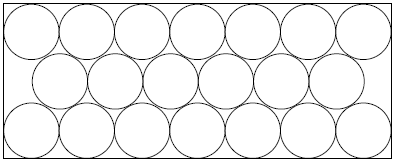
\includegraphics[scale=0.6]{AIME_2002I_Problem_02.png}
\end{center}

\textbf{88. (AIME 2002 I - P13) }In triangle $ABC$ the medians $\overline{AD}$ and $\overline{CE}$ have lengths $18$ and $27$, respectively, and $AB=24$. Extend $\overline{CE}$ to intersect the circumcircle of $ABC$ at $F$. The area of triangle $AFB$ is $m\sqrt{n}$, where $m$ and $n$ are positive integers and $n$ is not divisible by the square of any prime. Find $m+n$.\quad\textbf{Ans: 063}\\

\textbf{89. (AIME 2002 II - P14) }The perimeter of triangle $APM$ is $152$, and the angle $PAM$ is a right angle. A circle of radius $19$ with center $O$ on $\overline{AP}$ is drawn so that it is tangent to $\overline{AM}$ and $\overline{PM}$. Given that $OP=m/n$ where $m$ and $n$ are relatively prime positive integers, find $m+n$.\quad\textbf{Ans: 098}\\

\textbf{90. (AIME 2003 I - P5) }Consider the set of points that are inside or within one unit of a rectangular parallelepiped (box) that measures $3$ by $4$ by $5$ units. Given that the volume of this set is $\dfrac{m + n\pi}{p},$ where $m, n,$ and $p$ are positive integers, and $n$ and $p$ are relatively prime, find $m + n + p.$\quad\textbf{Ans: 505}\\

\textbf{91. (AIME 2003 I - P6) }The sum of the areas of all triangles whose vertices are also vertices of a $1$ by $1$ by $1$ cube is $m + \sqrt{n} + \sqrt{p},$ where $m, n,$ and $p$ are integers. Find $m + n + p.$\quad\textbf{Ans: 348}\\

\textbf{92. (AIME 2003 I - P7) }Point $B$ is on $\overline{AC}$ with $AB = 9$ and $BC = 21.$ Point $D$ is not on $\overline{AC}$ so that $AD = CD,$ and $AD$ and $BD$ are integers. Let $s$ be the sum of all possible perimeters of $\triangle ACD$. Find $s.$\quad\textbf{Ans: 380}\\

\textbf{93. (AIME 2003 I - P10) }Triangle $ABC$ is isosceles with $AC = BC$ and $\angle ACB = 106^\circ.$ Point $M$ is in the interior of the triangle so that $\angle MAC = 7^\circ$ and $\angle MCA = 23^\circ.$ Find the number of degrees in $\angle CMB.$\quad\textbf{Ans: $83^{\circ}$}\\

\textbf{94. (AIME 2003 I - P12) }In convex quadrilateral $ABCD, \angle A \cong \angle C, AB = CD = 180,$ and $AD \neq BC.$ The perimeter of $ABCD$ is 640. Find $\lfloor 1000 \cos A \rfloor.$ (The notation $\lfloor x \rfloor$ means the greatest integer that is less than or equal to $x.$)\quad\textbf{Ans: 777}\\

\textbf{95. (AIME 2003 I - P15) }In $\triangle ABC, AB = 360, BC = 507,$ and $CA = 780.$ Let $M$ be the midpoint of $\overline{CA},$ and let $D$ be the point on $\overline{CA}$ such that $\overline{BD}$ bisects angle $ABC.$ Let $F$ be the point on $\overline{BC}$ such that $\overline{DF} \perp \overline{BD}.$ Suppose that $\overline{DF}$ meets $\overline{BM}$ at $E.$ The ratio $DE: EF$ can be written in the form $m/n,$ where $m$ and $n$ are relatively prime positive integers. Find $m + n.$\quad\textbf{Ans: 289}\\

\textbf{96. (AIME 2004 I - P10) }A circle of radius 1 is randomly placed in a 15-by-36 rectangle $ABCD$ so that the circle lies completely within the rectangle. Given that the probability that the circle will not touch diagonal $AC$ is $m/n,$ where $m$ and $n$ are relatively prime positive integers. Find $m + n.$\quad\textbf{Ans: 817}\\

\textbf{97. (AIME 2004 I - P14) }A unicorn is tethered by a $20$-foot silver rope to the base of a magician's cylindrical tower whose radius is $8$ feet. The rope is attached to the tower at ground level and to the unicorn at a height of $4$ feet. The unicorn has pulled the rope taut, the end of the rope is $4$ feet from the nearest point on the tower, and the length of the rope that is touching the tower is $\dfrac{a-\sqrt{b}}c$ feet, where $a, b,$ and $c$ are positive integers, and $c$ is prime. Find $a+b+c.$\quad\textbf{Ans: 813}\\

\textbf{98. (AIME 2004 II - P1) }A chord of a circle is perpendicular to a radius at the midpoint of the radius. The ratio of the area of the larger of the two regions into which the chord divides the circle to the smaller can be expressed in the form $\dfrac{a\pi+b\sqrt{c}}{d\pi-e\sqrt{f}},$ where $a, b, c, d, e,$ and $f$ are positive integers, $a$ and $e$ are relatively prime, and neither $c$ nor $f$ is divisible by the square of any prime. Find the remainder when the product $abcdef$ is divided by 1000.\quad\textbf{Ans: 592}

\begin{center}
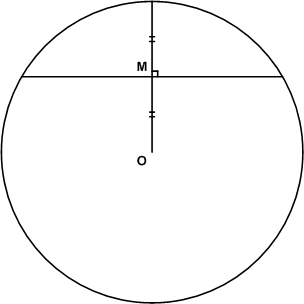
\includegraphics[scale=0.4]{2004_AIME_II_Problem_1.png}
\end{center}

\textbf{99. (AIME 2004 II - P7) }$ABCD$ is a rectangular sheet of paper that has been folded so that corner $B$ is matched with point $B'$ on edge $AD.$ The crease is $EF,$ where $E$ is on $AB$ and $F$ is on $CD.$ The dimensions $AE=8, BE=17,$ and $CF=3$ are given. The perimeter of rectangle $ABCD$ is $m/n,$ where $m$ and $n$ are relatively prime positive integers. Find $m+n.$\quad\textbf{Ans: 293}\\

\textbf{100. (AIME 2004 II - P11) }A right circular cone has a base with radius $600$ and height $200\sqrt{7}.$ A fly starts at a point on the surface of the cone whose distance from the vertex of the cone is $125$, and crawls along the surface of the cone to a point on the exact opposite side of the cone whose distance from the vertex is $375\sqrt{2}.$ Find the least distance that the fly could have crawled.\quad\textbf{Ans: 625}\\

\textbf{101. (AIME 2004 II - P12) }Let $ABCD$ be an isosceles trapezoid, whose dimensions are $AB = 6, BC=5=DA,$and $CD=4.$ Draw circles of radius 3 centered at $A$ and $B,$ and circles of radius 2 centered at $C$ and $D.$ A circle contained within the trapezoid is tangent to all four of these circles. Its radius is $\dfrac{-k+m\sqrt{n}}p,$ where $k, m, n,$ and $p$ are positive integers, $n$ is not divisible by the square of any prime, and $k$ and $p$ are relatively prime. Find $k+m+n+p.$\quad\textbf{Ans: 134}\\

\textbf{102. (AIME 2004 II - P13) }Let $ABCDE$ be a convex pentagon with $AB \parallel CE, BC \parallel AD, AC \parallel DE, \angle ABC=120^\circ, AB=3, BC=5,$ and $DE = 15.$ Given that the ratio between the area of triangle $ABC$ and the area of triangle $EBD$ is $m/n,$ where $m$ and $n$ are relatively prime positive integers, find $m+n.$\quad\textbf{Ans: 484}\\

\textbf{103. (AIME 2005 I - P1) }Six congruent circles form a ring with each circle externally tangent to two circles adjacent to it. All circles are internally tangent to a circle $C$ with radius 30. Let $K$ be the area of the region inside circle $C$ and outside of the six circles in the ring. Find $\lfloor K \rfloor$ (the floor function).\quad\textbf{Ans: 942} 

\begin{center}
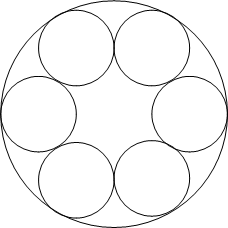
\includegraphics[scale=0.4]{2005_AIME_I_Problem_1.png}
\end{center}

\textbf{104. (AIME 2005 I - P10) }   Triangle $ABC$ lies in the cartesian plane and has an area of $70$. The coordinates of $B$ and $C$ are $(12,19)$ and $(23,20),$ respectively, and the coordinates of $A$ are $(p,q).$ The line containing the median to side $BC$ has slope $-5.$ Find the largest possible value of $p+q.$  \quad\textbf{Ans: 047 }

\begin{center}
\begin{asy}
import cse5;
import olympiad;
import graph;
size(100);
defaultpen(fontsize(8)); size(170); pair A=(15,32), B=(12,19), C=(23,20), M=B/2+C/2, P=(17,22); draw(A--B--C--A);draw(A--M);draw(B--P--C); label("A (p,q)",A,(1,1));label("B (12,19)",B,(-1,-1));label("C (23,20)",C,(1,-1));label("M",M,(0.2,-1)); label("(17,22)",P,(1,1)); dot(A^^B^^C^^M^^P);
\end{asy}
\end{center}

\textbf{105. (AIME 2005 I - P7) }  In quadrilateral $ABCD,\ BC=8,\ CD=12,\ AD=10,$ and $m\angle A= m\angle B = 60^\circ.$ Given that $AB = p + \sqrt{q},$ where $p$ and $q$ are positive integers, find $p+q.$  \quad\textbf{Ans: 150}\\

\textbf{106. (AIME 2005 I - P11) }   A semicircle with diameter $d$ is contained in a square whose sides have length 8. Given the maximum value of $d$ is $m - \sqrt{n},$ find $m+n.$  \quad\textbf{Ans: 544}\\

\textbf{107. (AIME 2005 I - P14) }  Consider the points $A(0,12), B(10,9), C(8,0),$ and $D(-4,7).$ There is a unique square $S$ such that each of the four points is on a different side of $S.$ Let $K$ be the area of $S.$ Find the remainder when $10K$ is divided by $1000$.  \quad\textbf{Ans: 936 }\\

\textbf{108. (AIME 2005 I - P15) }  Triangle $ABC$ has $BC=20.$ The incircle of the triangle evenly trisects the median $AD.$ If the area of the triangle is $m \sqrt{n}$ where $m$ and $n$ are integers and $n$ is not divisible by the square of a prime, find $m+n.$  \quad\textbf{Ans: 038}\\

\textbf{109. (AIME 2005 II - P8) }   Circles $C_1$ and $C_2$ are externally tangent, and they are both internally tangent to circle $C_3.$ The radii of $C_1$ and $C_2$ are 4 and 10, respectively, and the centers of the three circles are all collinear. A chord of $C_3$ is also a common external tangent of $C_1$ and $C_2.$ Given that the length of the chord is $\dfrac{m\sqrt{n}}p$ where $m,n,$ and $p$ are positive integers, $m$ and $p$ are relatively prime, and $n$ is not divisible by the square of any prime, find $m+n+p.$  \quad\textbf{Ans: 405}\\

\textbf{110. (AIME 2005 II - P10) }   Given that $O$ is a regular octahedron, that $C$ is the cube whose vertices are the centers of the faces of $O,$ and that the ratio of the volume of $O$ to that of $C$ is $\frac mn,$ where $m$ and $n$ are relatively prime integers, find $m+n.$  \quad\textbf{Ans: 011}\\

\textbf{111. (AIME 2005 II - P12) }   Square $ABCD$ has center $O,\ AB=900,\ E$ and $F$ are on $AB$ with $AE<BF$ and $E$ between $A$ and $F, m\angle EOF =45^\circ,$ and $EF=400.$ Given that $BF=p+q\sqrt{r},$ where $p,q,$ and $r$ are positive integers and $r$ is not divisible by the square of any prime, find $p+q+r.$  \quad\textbf{Ans: 307}\\

\textbf{112. (AIME 2005 II - P14) }   In triangle $ABC, AB=13, BC=15,$ and $CA = 14.$ Point $D$ is on $\overline{BC}$ with $CD=6.$ Point $E$ is on $\overline{BC}$ such that $\angle BAE\cong \angle CAD.$ Given that $BE=\dfrac{p}{q}$ where $p$ and $q$ are relatively prime positive integers, find $q.$  \quad\textbf{Ans: 463}\\

\textbf{113. (AIME 2005 II - P15) }   Let $w_1$ and $w_2$ denote the circles $x^2+y^2+10x-24y-87=0$ and $x^2 +y^2-10x-24y+153=0,$ respectively. Let $m$ be the smallest positive value of $a$ for which the line $y=ax$ contains the center of a circle that is externally tangent to $w_2$ and internally tangent to $w_1.$ Given that $m^2=\dfrac{p}{q}$ where $p$ and $q$ are relatively prime integers, find $p+q.$  \quad\textbf{Ans: 169}\\

\textbf{114. (AIME 2006 I - P6) }   In quadrilateral $ABCD$, $\angle B$ is a right angle, diagonal $\overline{AC}$ is perpendicular to $\overline{CD}$, $AB=18$, $BC=21$, and $CD=14$. Find the perimeter of $ABCD$.  \quad\textbf{Ans: 084}\\

\textbf{115. (AIME 2006 I - P7) }   An angle is drawn on a set of equally spaced parallel lines as shown. The ratio of the area of shaded region $\mathcal{C}$ to the area of shaded region $\mathcal{B}$ is 11/5. Find the ratio of shaded region $\mathcal{D}$ to the area of shaded region $\mathcal{A}.$  \quad\textbf{Ans: 408 }

\begin{center}
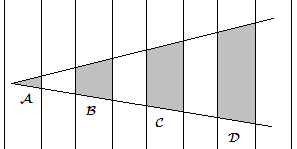
\includegraphics[scale=0.4]{2006AimeA7.PNG}
\end{center}

\textbf{116. (AIME 2006 I - P8) }  Hexagon $ABCDEF$ is divided into five rhombuses, $\mathcal{P, Q, R, S,}$ and $\mathcal{T,}$ as shown. Rhombuses $\mathcal{P, Q, R,}$ and $\mathcal{S}$ are congruent, and each has area $\sqrt{2006}.$ Let $K$ be the area of rhombus $\mathcal{T}$. Given that $K$ is a positive integer, find the number of possible values for $K$. \quad\textbf{Ans: 089}

\begin{center}
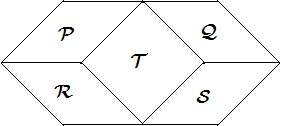
\includegraphics[scale=0.4]{2006AimeA8.PNG}
\end{center}

\textbf{117. (AIME 2006 I - P10) }   Eight circles of diameter 1 are packed in the first quadrant of the coordinate plane as shown. Let region $\mathcal{R}$ be the union of the eight circular regions. Line $l,$ with slope 3, divides $\mathcal{R}$ into two regions of equal area. Line $l$'s equation can be expressed in the form $ax=by+c,$ where $a, b,$ and $c$ are positive integers whose greatest common divisor is 1. Find $a^2+b^2+c^2.$  \quad\textbf{Ans: 065}

\begin{center}
\begin{asy}
import cse5;
import olympiad;
import graph;
size(120);defaultpen(linewidth(0.7)); draw((6.5,0)--origin--(0,6.5), Arrows(5)); int[] array={3,3,2}; int i,j; for(i=0; i<3; i=i+1) { for(j=0; j<array[i]; j=j+1) { draw(Circle((1+2*i,1+2*j),1)); }} label("x", (7,0)); label("y", (0,7));
\end{asy}
\end{center}

\textbf{118. (AIME 2006 I - P14) }   A tripod has three legs each of length $5$ feet. When the tripod is set up, the angle between any pair of legs is equal to the angle between any other pair, and the top of the tripod is $4$ feet from the ground. In setting up the tripod, the lower 1 foot of one leg breaks off. Let $h$ be the height in feet of the top of the tripod from the ground when the broken tripod is set up. Then $h$ can be written in the form $\dfrac m{\sqrt{n}},$ where $m$ and $n$ are positive integers and $n$ is not divisible by the square of any prime. Find $\lfloor m+\sqrt{n}\rfloor.$ (The notation $\lfloor x\rfloor$ denotes the greatest integer that is less than or equal to $x.$)  \quad\textbf{Ans: 183}\\

\textbf{119. (AIME 2006 II - P1) }   In convex hexagon $ABCDEF$, all six sides are congruent, $\angle A$ and $\angle D$ are right angles, and $\angle B, \angle C, \angle E,$ and $\angle F$ are congruent. The area of the hexagonal region is $2116(\sqrt{2}+1).$ Find $AB$.  \quad\textbf{Ans: 006 }\\

\textbf{120. (AIME 2006 II - P2) }   The lengths of the sides of a triangle with positive area are $\log_{10} 12$, $\log_{10} 75$, and $\log_{10} n$, where $n$ is a positive integer. Find the number of possible values for $n$.  \quad\textbf{Ans: 893}\\

\textbf{121. (AIME 2006 II - P6) }  Square $ABCD$ has sides of length 1. Points $E$ and $F$ are on $\overline{BC}$ and $\overline{CD},$ respectively, so that $\triangle AEF$ is equilateral. A square with vertex $B$ has sides that are parallel to those of $ABCD$ and a vertex on $\overline{AE}.$ The length of a side of this smaller square is $\dfrac{a-\sqrt{b}}{c},$ where $a, b,$ and $c$ are positive integers and $b$ is not divisible by the square of any prime. Find $a+b+c.$  \quad\textbf{Ans: 012}\\

\textbf{122. (AIME 2006 II - P9) }   Circles $\mathcal{C}_1, \mathcal{C}_2,$ and $\mathcal{C}_3$ have their centers at (0,0), (12,0), and (24,0), and have radii 1, 2, and 4, respectively. Line $t_1$ is a common internal tangent to $\mathcal{C}_1$ and $\mathcal{C}_2$ and has a positive slope, and line $t_2$ is a common internal tangent to $\mathcal{C}_2$ and $\mathcal{C}_3$ and has a negative slope. Given that lines $t_1$ and $t_2$ intersect at $(x,y),$ and that $x=p-q\sqrt{r},$ where $p, q,$ and $r$ are positive integers and $r$ is not divisible by the square of any prime, find $p+q+r.$  \quad\textbf{Ans: 027}\\

\textbf{123. (AIME 2006 II - P12) }   Equilateral $\triangle ABC$ is inscribed in a circle of radius $2$. Extend $\overline{AB}$ through $B$ to point $D$ so that $AD=13,$ and extend $\overline{AC}$ through $C$ to point $E$ so that $AE = 11.$ Through $D,$ draw a line $l_1$ parallel to $\overline{AE},$ and through $E,$ draw a line $l_2$ parallel to $\overline{AD}.$ Let $F$ be the intersection of $l_1$ and $l_2.$ Let $G$ be the point on the circle that is collinear with $A$ and $F$ and distinct from $A.$ Given that the area of $\triangle CBG$ can be expressed in the form $\dfrac{p\sqrt{q}}{r},$ where $p, q,$ and $r$ are positive integers, $p$ and $r$ are relatively prime, and $q$ is not divisible by the square of any prime, find $p+q+r.$  \quad\textbf{Ans: 865}\\

\textbf{124. (AIME 2007 I - P9) }   In right triangle $ABC$ with right angle $C$, $CA = 30$ and $CB = 16$. Its legs $CA$ and $CB$ are extended beyond $A$ and $B$. Points $O_1$ and $O_2$ lie in the exterior of the triangle and are the centers of two circles with equal radii. The circle with center $O_1$ is tangent to the hypotenuse and to the extension of leg $CA$, the circle with center $O_2$ is tangent to the hypotenuse and to the extension of leg $CB$, and the circles are externally tangent to each other. The length of the radius either circle can be expressed as $p/q$, where $p$ and $q$ are relatively prime positive integers. Find $p+q$.  \quad\textbf{Ans: 737}

\begin{center}
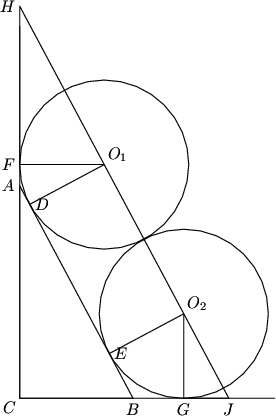
\includegraphics[scale=0.3]{AIME_I_2007-9.png}
\end{center}

\textbf{125. (AIME 2007 I - P12) }   In isosceles triangle $\triangle ABC$, $A$ is located at the origin and $B$ is located at $(20,0)$. Point $C$ is in the first quadrant with $AC = BC$ and angle $BAC = 75^{\circ}$. If triangle $ABC$ is rotated counterclockwise about point $A$ until the image of $C$ lies on the positive $y$-axis, the area of the region common to the original and the rotated triangle is in the form $p\sqrt{2} + q\sqrt{3} + r\sqrt{6} + s$, where $p,q,r,s$ are integers. Find $\dfrac{p-q+r-s}2$. \quad\textbf{Ans: 875}

\begin{center}
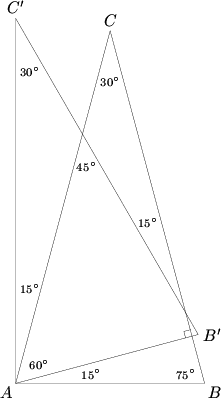
\includegraphics[scale=0.3]{AIME_I_2007-12.png}
\end{center}

\textbf{126. (AIME 2007 I - P13) }   A square pyramid with base $ABCD$ and vertex $E$ has eight edges of length $4$. A plane passes through the midpoints of $AE$, $BC$, and $CD$. The plane's intersection with the pyramid has an area that can be expressed as $\sqrt{p}$. Find $p$.  \quad\textbf{Ans: 080}

\begin{center}
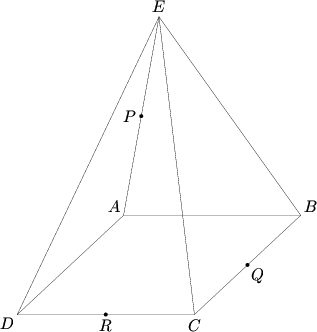
\includegraphics[scale=0.4]{AIME_I_2007-13.png}
\end{center}


\textbf{127. (AIME 2007 I - P15) }   Let $ABC$ be an equilateral triangle, and let $D$ and $F$ be points on sides $BC$ and $AB$, respectively, with $FA = 5$ and $CD = 2$. Point $E$ lies on side $CA$ such that angle $DEF = 60^{\circ}$. The area of triangle $DEF$ is $14\sqrt{3}$. The two possible values of the length of side $AB$ are $p \pm q \sqrt{r}$, where $p$ and $q$ are rational, and $r$ is an integer not divisible by the square of a prime. Find $r$.  \quad\textbf{Ans: 989}\\

\textbf{128. (AIME 2007 II - P3) }   Square $ABCD$ has side length $13$, and points $E$ and $F$ are exterior to the square such that $BE=DF=5$ and $AE=CF=12$. Find $EF^{2}$. \quad\textbf{Ans: 578}
  
\begin{center}
\begin{asy}
import cse5;
import olympiad;
import graph;
unitsize(0.2 cm);  pair A, B, C, D, E, F;  A = (0,13); B = (13,13); C = (13,0); D = (0,0); E = A + (12*12/13,5*12/13); F = D + (5*5/13,-5*12/13);  draw(A--B--C--D--cycle); draw(A--E--B); draw(C--F--D);  dot("$A$", A, W); dot("$B$", B, dir(0)); dot("$C$", C, dir(0)); dot("$D$", D, W); dot("$E$", E, N); dot("$F$", F, S);
\end{asy}
\end{center}

\textbf{129. (AIME 2007 II - P9) }   Rectangle $ABCD$ is given with $AB=63$ and $BC=448.$ Points $E$ and $F$ lie on $AD$ and $BC$ respectively, such that $AE=CF=84.$ The inscribed circle of triangle $BEF$ is tangent to $EF$ at point $P,$ and the inscribed circle of triangle $DEF$ is tangent to $EF$ at point $Q.$ Find $PQ.$ \quad\textbf{Ans: 259 }

\begin{center}
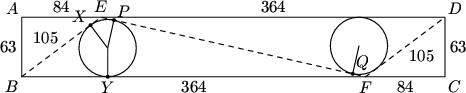
\includegraphics[scale=0.6]{2007_AIME_II-9.png}
\end{center}

\textbf{130. (AIME 2007 II - P15) }   Four circles $\omega,$ $\omega_{A},$ $\omega_{B},$ and $\omega_{C}$ with the same radius are drawn in the interior of triangle $ABC$ such that $\omega_{A}$ is tangent to sides $AB$ and $AC$, $\omega_{B}$ to $BC$ and $BA$, $\omega_{C}$ to $CA$ and $CB$, and $\omega$ is externally tangent to $\omega_{A},$ $\omega_{B},$ and $\omega_{C}$. If the sides of triangle $ABC$ are $13,$ $14,$ and $15,$ the radius of $\omega$ can be represented in the form $\frac{m}{n}$, where $m$ and $n$ are relatively prime positive integers. Find $m+n.$  \quad\textbf{Ans: 389}\\

\textbf{131. (AIME 2008 I - P5) }   A right circular cone has base radius $r$ and height $h$. The cone lies on its side on a flat table. As the cone rolls on the surface of the table without slipping, the point where the cone's base meets the table traces a circular arc centered at the point where the vertex touches the table. The cone first returns to its original position on the table after making $17$ complete rotations. The value of $h/r$ can be written in the form $m\sqrt {n}$, where $m$ and $n$ are positive integers and $n$ is not divisible by the square of any prime. Find $m + n$.  \quad\textbf{Ans: 014}\\

\textbf{132. (AIME 2008 I - P10) }   Let $ABCD$ be an isosceles trapezoid with $\overline{AD}||\overline{BC}$ whose angle at the longer base $\overline{AD}$ is $\dfrac{\pi}{3}$. The diagonals have length $10\sqrt {21}$, and point $E$ is at distances $10\sqrt {7}$ and $30\sqrt {7}$ from vertices $A$ and $D$, respectively. Let $F$ be the foot of the altitude from $C$ to $\overline{AD}$. The distance $EF$ can be expressed in the form $m\sqrt {n}$, where $m$ and $n$ are positive integers and $n$ is not divisible by the square of any prime. Find $m + n$.  \quad\textbf{Ans: 032}\\

\textbf{133. (AIME 2008 I - P15) }   Let $\overline{AB}$ be a diameter of circle $\omega$. Extend $\overline{AB}$ through $A$ to $C$. Point $T$ lies on $\omega$ so that line $CT$ is tangent to $\omega$. Point $P$ is the foot of the perpendicular from $A$ to line $CT$. Suppose $AB = 18$, and let $m$ denote the maximum possible length of segment $BP$. Find $m^{2}$.  \quad\textbf{Ans: 871}

\begin{center}
\begin{asy}
import cse5;
import olympiad;
import graph;
 size(120); pathpen=black; real s=sqrt(17); real r=(sqrt(51)+s)/sqrt(2); D((0,2*s)--(0,0)--(2*s,0)); D((0,s)--r*dir(45)--(s,0)); D((0,0)--r*dir(45)); D((r*dir(45).x,2*s)--r*dir(45)--(2*s,r*dir(45).y)); MP("30^\circ",r*dir(45)-(0.25,1),SW); MP("30^\circ",r*dir(45)-(1,0.5),SW); MP("\sqrt{17}",(0,s/2),W); MP("\sqrt{17}",(s/2,0),S); MP("\mathrm{cut}",((0,s)+r*dir(45))/2,N); MP("\mathrm{cut}",((s,0)+r*dir(45))/2,E); MP("\mathrm{fold}",(r*dir(45).x,s+r/2*dir(45).y),E); MP("\mathrm{fold}",(s+r/2*dir(45).x,r*dir(45).y));
\end{asy}
\end{center}

\textbf{135. (AIME 2008 II - P5) }   In trapezoid $ABCD$ with $\overline{BC}\parallel\overline{AD}$, let $BC = 1000$ and $AD = 2008$. Let $\angle A = 37^\circ$, $\angle D = 53^\circ$, and $M$ and $N$ be the midpoints of $\overline{BC}$ and $\overline{AD}$, respectively. Find the length $MN$.  \quad\textbf{Ans: 504}\\

\textbf{136. (AIME 2008 II - P11) }   In triangle $ABC$, $AB = AC = 100$, and $BC = 56$. Circle $P$ has radius $16$ and is tangent to $\overline{AC}$ and $\overline{BC}$. Circle $Q$ is externally tangent to $P$ and is tangent to $\overline{AB}$ and $\overline{BC}$. No point of circle $Q$ lies outside of $\triangle ABC$. The radius of circle $Q$ can be expressed in the form $m - n\sqrt {k}$, where $m$, $n$, and $k$ are positive integers and $k$ is the product of distinct primes. Find $m + nk$.  \quad\textbf{Ans: 254}\\

\textbf{137. (AIME 2008 II - P13) }   A regular hexagon with center at the origin in the complex plane has opposite pairs of sides one unit apart. One pair of sides is parallel to the imaginary axis. Let $R$ be the region outside the hexagon, and let $S = \left\lbrace\dfrac{1}{z}|z \in R\right\rbrace$. Then the area of $S$ has the form $a\pi + \sqrt{b}$, where $a$ and $b$ are positive integers. Find $a + b$.  \quad\textbf{Ans: 029}\\

\textbf{138. (AIME 2009 I - P5) }   Triangle $ABC$ has $AC = 450$ and $BC = 300$. Points $K$ and $L$ are located on $\overline{AC}$ and $\overline{AB}$ respectively so that $AK = CK$, and $\overline{CL}$ is the angle bisector of angle $C$. Let $P$ be the point of intersection of $\overline{BK}$ and $\overline{CL}$, and let $M$ be the point on line $BK$ for which $K$ is the midpoint of $\overline{PM}$. If  $AM = 180$, find $LP$.  \quad\textbf{Ans: 072}\\


\textbf{139. (AIME 2010 I - P11) }   Let $\mathcal{R}$ be the region consisting of the set of points in the coordinate plane that satisfy both $|8 - x| + y \le 10$ and $3y - x \ge 15$. When $\mathcal{R}$ is revolved around the line whose equation is $3y - x = 15$, the volume of the resulting solid is $\dfrac {m\pi}{n\sqrt {p}}$, where $m$, $n$, and $p$ are positive integers, $m$ and $n$ are relatively prime, and $p$ is not divisible by the square of any prime. Find $m + n + p$.  \quad\textbf{Ans: 365}\\


\textbf{140. (AIME 2010 I - P13) }   Rectangle $ABCD$ and a semicircle with diameter $AB$ are coplanar and have nonoverlapping interiors. Let $\mathcal{R}$ denote the region enclosed by the semicircle and the rectangle. Line $\ell$ meets the semicircle, segment $AB$, and segment $CD$ at distinct points $N$, $U$, and $T$, respectively. Line $\ell$ divides region $\mathcal{R}$ into two regions with areas in the ratio $1: 2$. Suppose that $AU = 84$, $AN = 126$, and $UB = 168$. Then $DA$ can be represented as $m\sqrt {n}$, where $m$ and $n$ are positive integers and $n$ is not divisible by the square of any prime. Find $m + n$.  \quad\textbf{Ans: 069}\\


\textbf{141. (AIME 2010 I - P15) }   In $\triangle{ABC}$ with $AB = 12$, $BC = 13$, and $AC = 15$, let $M$ be a point on $\overline{AC}$ such that the incircles of $\triangle{ABM}$ and $\triangle{BCM}$ have equal radii. Let $p$ and $q$ be positive relatively prime integers such that $\frac {AM}{CM} = \dfrac {p}{q}$. Find $p + q$.  \quad\textbf{Ans: 045}\\


\textbf{142. (AIME 2010 II - P9) }   Let $ABCDEF$ be a regular hexagon. Let $G$, $H$, $I$, $J$, $K$, and $L$ be the midpoints of sides $AB$, $BC$, $CD$, $DE$, $EF$, and $AF$, respectively. The segments $\overline{AH}$, $\overline{BI}$, $\overline{CJ}$, $\overline{DK}$, $\overline{EL}$, and $\overline{FG}$ bound a smaller regular hexagon. Let the ratio of the area of the smaller hexagon to the area of $ABCDEF$ be expressed as a fraction $\dfrac {m}{n}$ where $m$ and $n$ are relatively prime positive integers. Find $m + n$.  \quad\textbf{Ans: 011}\\


\textbf{143. (AIME 2010 II - P12) }   Two noncongruent integer-sided isosceles triangles have the same perimeter and the same area. The ratio of the lengths of the bases of the two triangles is $8: 7$. Find the minimum possible value of their common perimeter.  \quad\textbf{Ans: 676}\\


\textbf{144. (AIME 2010 II - P14) }   Triangle $ABC$ with right angle at $C$, $\angle BAC < 45^\circ$ and $AB = 4$. Point $P$ on $\overline{AB}$ is chosen such that $\angle APC = 2\angle ACP$ and $CP = 1$. The ratio $\frac{AP}{BP}$ can be represented in the form $p + q\sqrt{r}$, where $p$, $q$, $r$ are positive integers and $r$ is not divisible by the square of any prime. Find $p+q+r$.  \quad\textbf{Ans: 007}\\


\textbf{145. (AIME 2011 I - P8) }   In triangle $ABC$, $BC = 23$, $CA = 27$, and $AB = 30$. Points $V$ and $W$ are on $\overline{AC}$ with $V$ on $\overline{AW}$, points $X$ and $Y$ are on $\overline{BC}$ with $X$ on $\overline{CY}$, and points $Z$ and $U$ are on $\overline{AB}$ with $Z$ on $\overline{BU}$. In addition, the points are positioned so that $\overline{UV}\parallel\overline{BC}$, $\overline{WX}\parallel\overline{AB}$, and $\overline{YZ}\parallel\overline{CA}$. Right angle folds are then made along $\overline{UV}$, $\overline{WX}$, and $\overline{YZ}$. The resulting figure is placed on a level floor to make a table with triangular legs. Let $h$ be the maximum possible height of a table constructed from triangle $ABC$ whose top is parallel to the floor. Then $h$ can be written in the form $\dfrac{k\sqrt{m}}{n}$, where $k$ and $n$ are relatively prime positive integers and $m$ is a positive integer that is not divisible by the square of any prime. Find   \quad\textbf{Ans: 318}

\begin{center}
\begin{asy}
import cse5;
import olympiad;
import graph;
unitsize(1 cm); pair translate; pair[] A, B, C, U, V, W, X, Y, Z; A[0] = (1.5,2.8); B[0] = (3.2,0); C[0] = (0,0); U[0] = (0.69*A[0] + 0.31*B[0]); V[0] = (0.69*A[0] + 0.31*C[0]); W[0] = (0.69*C[0] + 0.31*A[0]); X[0] = (0.69*C[0] + 0.31*B[0]); Y[0] = (0.69*B[0] + 0.31*C[0]); Z[0] = (0.69*B[0] + 0.31*A[0]); translate = (7,0); A[1] = (1.3,1.1) + translate; B[1] = (2.4,-0.7) + translate; C[1] = (0.6,-0.7) + translate; U[1] = U[0] + translate; V[1] = V[0] + translate; W[1] = W[0] + translate; X[1] = X[0] + translate; Y[1] = Y[0] + translate; Z[1] = Z[0] + translate; draw (A[0]--B[0]--C[0]--cycle); draw (U[0]--V[0],dashed); draw (W[0]--X[0],dashed); draw (Y[0]--Z[0],dashed); draw (U[1]--V[1]--W[1]--X[1]--Y[1]--Z[1]--cycle); draw (U[1]--A[1]--V[1],dashed); draw (W[1]--C[1]--X[1]); draw (Y[1]--B[1]--Z[1]); dot("$A$",A[0],N); dot("$B$",B[0],SE); dot("$C$",C[0],SW); dot("$U$",U[0],NE); dot("$V$",V[0],NW); dot("$W$",W[0],NW); dot("$X$",X[0],S); dot("$Y$",Y[0],S); dot("$Z$",Z[0],NE); dot(A[1]); dot(B[1]); dot(C[1]); dot("$U$",U[1],NE); dot("$V$",V[1],NW); dot("$W$",W[1],NW); dot("$X$",X[1],dir(-70)); dot("$Y$",Y[1],dir(250)); dot("$Z$",Z[1],NE);
\end{asy}
\end{center}

\textbf{146. (AIME 2011 I - P13) }   A cube with side length 10 is suspended above a plane. The vertex closest to the plane is labeled $A$. The three vertices adjacent to vertex $A$ are at heights 10, 11, and 12 above the plane. The distance from vertex $A$ to the plane can be expressed as $\dfrac{r-\sqrt{s}}{t}$, where $r$, $s$, and $t$ are positive integers, and $r+s+t<{1000}$. Find $r+s+t$.  \quad\textbf{Ans: 330}\\

\textbf{147. (AIME 2011  II - P1) }   Gary purchased a large beverage, but only drank $m/n$ of it, where $m$ and $n$ are relatively prime positive integers. If he had purchased half as much and drunk twice as much, he would have wasted only $2/9$ as much beverage. Find $m+n$.  \quad\textbf{Ans: 037}\\

\textbf{148. (AIME 2011 II - P2) }   On square $ABCD$, point $E$ lies on side $AD$ and point $F$ lies on side $BC$, so that $BE=EF=FD=30$. Find the area of the square $ABCD$.  \quad\textbf{Ans: 810}\\

\textbf{149. (AIME 2011 II - P3) }   The degree measures of the angles in a convex 18-sided polygon form an increasing arithmetic sequence with integer values. Find the degree measure of the smallest angle.  \quad\textbf{Ans: 143}\\

\textbf{150. (AIME 2011 II - P4) }   In triangle $ABC$, $AB=\frac{20}{11} AC$. The angle bisector of $\angle A$ intersects $BC$ at point $D$, and point $M$ is the midpoint of $AD$. Let $P$ be the point of the intersection of $AC$ and $BM$. The ratio of $CP$ to $PA$ can be expressed in the form $\dfrac{m}{n}$, where $m$ and $n$ are relatively prime positive integers. Find $m+n$.  \quad\textbf{Ans: 051}\\

\textbf{151. (AIME 2011 II - P10) }   A circle with center $O$ has radius 25. Chord $\overline{AB}$ of length 30 and chord $\overline{CD}$ of length 14 intersect at point $P$. The distance between the midpoints of the two chords is 12. The quantity $OP^2$ can be represented as $\dfrac{m}{n}$, where $m$ and $n$ are relatively prime positive integers. Find the remainder when $m + n$ is divided by 1000.  \quad\textbf{Ans: 057}\\

\textbf{152. (AIME 2011 II - P13) }   Point $P$ lies on the diagonal $AC$ of square $ABCD$ with $AP > CP$. Let $O_{1}$ and $O_{2}$ be the circumcenters of triangles $ABP$ and $CDP$ respectively. Given that $AB = 12$ and $\angle O_{1}PO_{2} = 120^{\circ}$, then $AP = \sqrt{a} + \sqrt{b}$, where $a$ and $b$ are positive integers. Find $a + b$.  \quad\textbf{Ans: 096}\\

\textbf{153. (AIME 2012 I - P8) }   Cube $ABCDEFGH,$ labeled as shown below, has edge length $1$ and is cut by a plane passing through vertex $D$ and the midpoints $M$ and $N$ of $\overline{AB}$ and $\overline{CG}$ respectively. The plane divides the cube into two solids. The volume of the larger of the two solids can be written in the form $\dfrac{p}{q},$ where $p$ and $q$ are relatively prime positive integers. Find $p+q.$  \quad\textbf{Ans: 089}

\begin{center}
\begin{asy}
import cse5;
import olympiad;
import graph;
unitsize(6mm); pathpen=black; dotfactor=3;  pair A = (0,0), B = (3.8,0), C = (5.876,1.564), D = (2.076,1.564), E = (0,3.8), F = (3.8,3.8), G = (5.876,5.364), H = (2.076,5.364), M = (1.9,0), N = (5.876,3.465); pair[] dotted = {A,B,C,D,E,F,G,H,M,N};  D(A--B--C--G--H--E--A); D(E--F--B); D(F--G); pathpen=dashed; D(A--D--H); D(D--C);  dot(dotted); label("$A$",A,SW); label("$B$",B,S); label("$C$",C,SE); label("$D$",D,NW); label("$E$",E,W); label("$F$",F,SE); label("$G$",G,NE); label("$H$",H,NW); label("$M$",M,S); label("$N$",N,NE); 
\end{asy}
\end{center}

\textbf{154. (AIME 2013 I - P7) }   A rectangular box has width $12$ inches, length $16$ inches, and height $\dfrac{m}{n}$ inches, where $m$ and $n$ are relatively prime positive integers. Three faces of the box meet at a corner of the box. The center points of those three faces are the vertices of a triangle with an area of $30$ square inches. Find $m+n$.  \quad\textbf{Ans: 041}\\

\textbf{155. (AIME 2014 II - P8) }   Circle $C$ with radius 2 has diameter $\overline{AB}$. Circle D is internally tangent to circle $C$ at $A$. Circle $E$ is internally tangent to circle $C$, externally tangent to circle $D$, and tangent to $\overline{AB}$. The radius of circle $D$ is three times the radius of circle $E$, and can be written in the form $\sqrt{m}-n$, where $m$ and $n$ are positive integers. Find $m+n$.  \quad\textbf{Ans: 254}\\

\textbf{156. (AIME 2014 II - P11) }   n $\triangle RED$, $\measuredangle DRE=75^{\circ}$ and $\measuredangle RED=45^{\circ}$. $|RD|=1$. Let $M$ be the midpoint of segment $\overline{RD}$. Point $C$ lies on side $\overline{ED}$ such that $\overline{RC}\perp\overline{EM}$. Extend segment $\overline{DE}$ through $E$ to point $A$ such that $CA=AR$. Then $AE=\dfrac{a-\sqrt{b}}{c}$, where $a$ and $c$ are relatively prime positive integers, and $b$ is a positive integer. Find $a+b+c$.  \quad\textbf{Ans: 056}\\

\textbf{157. (AIME 2015 I - P11) }   Triangle $ABC$ has positive integer side lengths with $AB=AC$. Let $I$ be the intersection of the bisectors of $\angle B$ and $\angle C$. Suppose $BI=8$. Find the smallest possible perimeter of $\triangle ABC$.  \quad\textbf{Ans: 108}\\

\textbf{158. (AIME 2015 I - P13) }   With all angles measured in degrees, the product $\prod_{k=1}^{45} \csc^2(2k-1)^\circ=m^n$, where $m$ and $n$ are integers greater than 1. Find $m+n$.  \quad\textbf{Ans: 091}\\

\textbf{159. (AIME 2015 I - P15) }   A block of wood has the shape of a right circular cylinder with radius $6$ and height $8$, and its entire surface has been painted blue. Points $A$ and $B$ are chosen on the edge of one of the circular faces of the cylinder so that $AB$ on that face measures $120^\text{o}$. The block is then sliced in half along the plane that passes through point $A$, point $B$, and the center of the cylinder, revealing a flat, unpainted face on each half. The area of one of these unpainted faces is $a\cdot\pi + b\sqrt{c}$, where $a$, $b$, and $c$ are integers and $c$ is not divisible by the square of any prime. Find $a+b+c$. \quad\textbf{Ans: 053}

\begin{center}
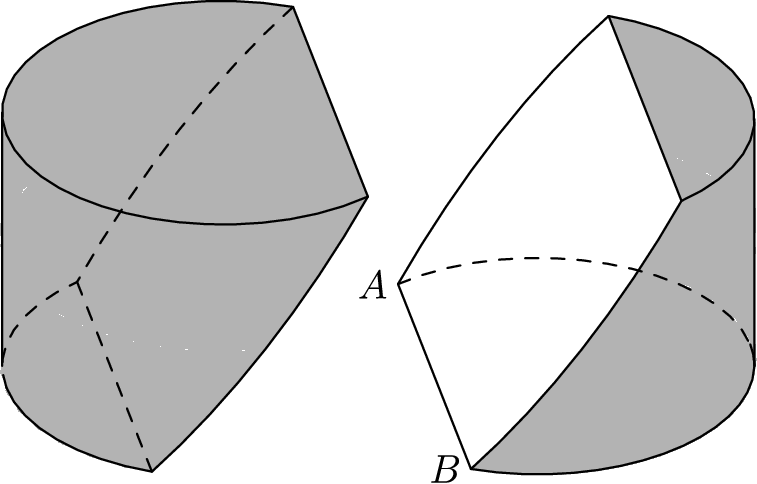
\includegraphics[scale=0.4]{AIME_I_2015-15.png}
\end{center}

\textbf{160. (AIME 2015 II - P9) }   A cylindrical barrel with radius $4$ feet and height $10$ feet is full of water. A solid cube with side length $8$ feet is set into the barrel so that the diagonal of the cube is vertical. The volume of water thus displaced is $v$ cubic feet. Find $v^2$.  \quad\textbf{Ans: 384}

\begin{center}
\begin{asy}
import cse5;
import olympiad;
import graph; 
import three;
import solids;
size(5cm); currentprojection=orthographic(1,-1/6,1/6);  draw(surface(revolution((0,0,0),(-2,-2*sqrt(3),0)--(-2,-2*sqrt(3),-10),Z,0,360)),white,nolight);  triple A =(8*sqrt(6)/3,0,8*sqrt(3)/3), B = (-4*sqrt(6)/3,4*sqrt(2),8*sqrt(3)/3), C = (-4*sqrt(6)/3,-4*sqrt(2),8*sqrt(3)/3), X = (0,0,-2*sqrt(2));  draw(X--X+A--X+A+B--X+A+B+C); draw(X--X+B--X+A+B); draw(X--X+C--X+A+C--X+A+B+C); draw(X+A--X+A+C); draw(X+C--X+C+B--X+A+B+C,linetype("2 4")); draw(X+B--X+C+B,linetype("2 4"));  draw(surface(revolution((0,0,0),(-2,-2*sqrt(3),0)--(-2,-2*sqrt(3),-10),Z,0,240)),white,nolight); draw((-2,-2*sqrt(3),0)..(4,0,0)..(-2,2*sqrt(3),0)); draw((-4*cos(atan(5)),-4*sin(atan(5)),0)--(-4*cos(atan(5)),-4*sin(atan(5)),-10)..(4,0,-10)..(4*cos(atan(5)),4*sin(atan(5)),-10)--(4*cos(atan(5)),4*sin(atan(5)),0)); draw((-2,-2*sqrt(3),0)..(-4,0,0)..(-2,2*sqrt(3),0),linetype("2 4")); 
\end{asy}
\end{center}

\textbf{161. (AIME 2016 II - P14) }   Equilateral $\triangle ABC$ has side length $600$. Points $P$ and $Q$ lie outside the plane of $\triangle ABC$ and are on opposite sides of the plane. Furthermore, $PA=PB=PC$, and $QA=QB=QC$, and the planes of $\triangle PAB$ and $\triangle QAB$ form a $120^{\circ}$ dihedral angle (the angle between the two planes). There is a point $O$ whose distance from each of $A,B,C,P,$ and $Q$ is $d$. Find $d$.  \quad\textbf{Ans: 450}

\end{document}